Now that we have fitted our data $\{Y_t\}$ to a suitable model, the next
reasonable step is to use the model to provide a forecast of the next 48 hour cycle
,i.e. for the time period of 2015-11-28 21:00 EST - 2015-11-30 21:00 EST.

The programming language R provides many tools to forecast data. One such tool
is the \texttt{forecast} package, which we employ. Using the model provided by
\eqref{sarima_model}, we provide the model in an acceptable form to the
function \texttt{predict} as well as the desired number of lags, e.g. 48,
and arrive at the forecasted values. As the model is for the transformed data
$Y_t = \log(X_t) - E(\log(X_t))$, we must apply the inverse transformation to the
forecasted values. Doing so gives us the table of values found in Appendix
\ref{forecast_table} along with 90\% confidence intervals. A plot of these
forecasts combined with the original data can be found in Figure \ref{forecast_plot}.

\begin{figure}[!h]
  \centerline{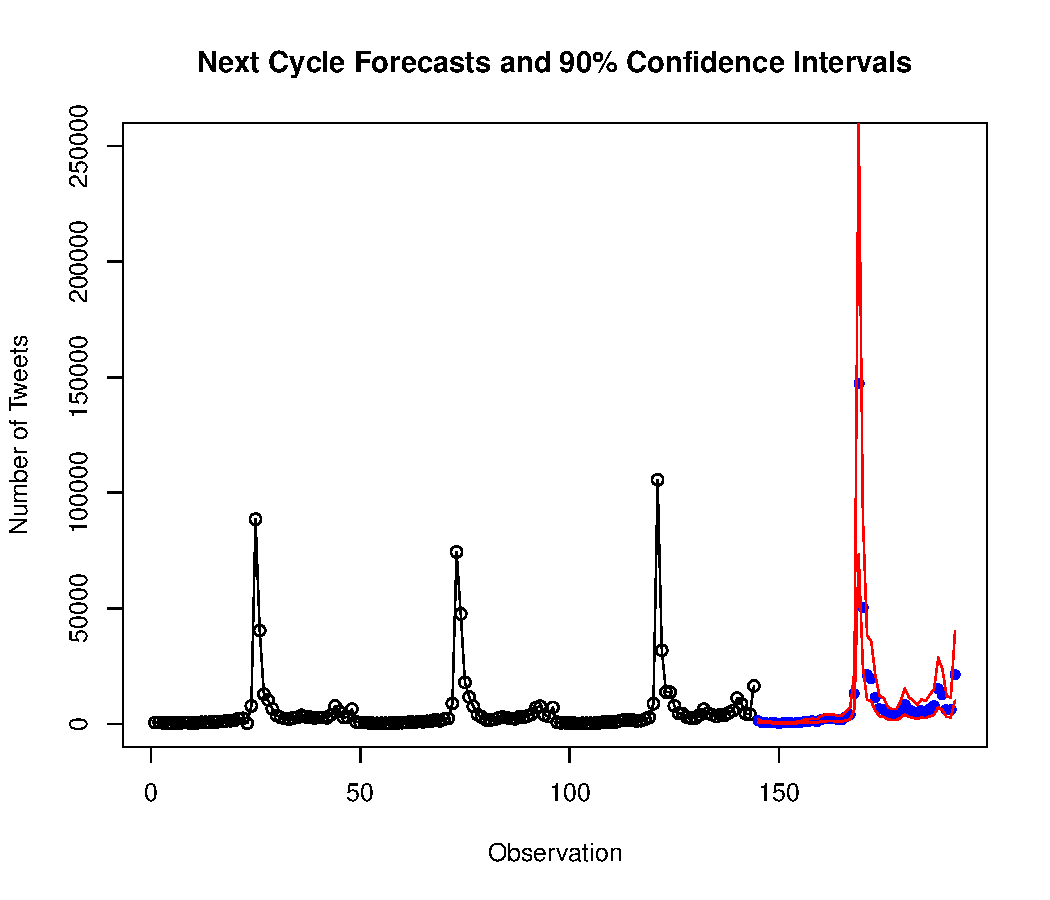
\includegraphics[scale=0.75]{../analysis/plots/forecast}}
  \caption{Plot of forecasted data for the next 48 cycle for data $X_t$.}\label{forecast_plot}
\end{figure}

The shape of the forecast seems to follow the same shape as the previous cycles
suggesting that the forecasts seem plausible. Also note the sensitivity of
the forecast at the time of interest, i.e. at 2015-11-29 21:00 EST.